\chapter{Comunicazione e protocollo}
\label{cap:comunicazione}

La comunicazione tra i tre nodi del sistema (PC, Board A e Board B) avviene esclusivamente attraverso canali UART seriali. Questo capitolo descrive il protocollo applicativo progettato per veicolare messaggi di natura diversa (immagini, ritagli, stringhe alfanumeriche, segnali di sincronizzazione)  sopra un mezzo fisico orientato a un flusso di byte privo di struttura intrinseca.

\section{Configurazione UART}
\label{sec:uart-config}

Tutti e tre i canali del sistema (PC$\leftrightarrow$A, A$\leftrightarrow$B) operano alla stessa velocità di 115\,200~baud in modalità 8N1 (8 bit di dato, nessun bit di parità, 1 bit di stop), senza controllo di flusso hardware. La scelta di un baud rate moderato è motivata dalla volontà di garantire affidabilità: a 115\,200~baud i due microcontrollori sostengono la comunicazione senza errori, mentre velocità superiori richiederebbero una sintonizzazione fine della FPLL del clock UART. Su entrambe le board, la USART2 è configurata attraverso un file \textit{overlay} devicetree che dichiara lo stato del dispositivo, la velocità di trasferimento e il \textit{pin control} per mappare i segnali sulle uscite fisiche PD5 (TX) e PD6 (RX).

\begin{lstlisting}[style=stileDevicetree, caption={Overlay devicetree per l'abilitazione della USART2 con clock a 115\,200~baud.}, label={lst:overlay}]
/ {
    chosen {
        zephyr,sram = &sram0;
    };
};

&sram0 {
    reg = <0x24000000 0x80000>;
};

&usart2 {
    status = "okay";
    current-speed = <115200>;
    pinctrl-0 = <&usart2_tx_pd5 &usart2_rx_pd6>;
    pinctrl-names = "default";
};
\end{lstlisting}

Lo stesso file definisce anche la mappatura della SRAM principale all'indirizzo $\mathtt{0x24000000}$ con dimensione $\mathtt{0x80000}$ (512~KB): senza questa dichiarazione esplicita Zephyr utilizzerebbe la regione di default, che sulla H745 non corrisponde alla SRAM grande ma a un blocco più piccolo non sufficiente per ospitare le \textit{activation} dei modelli neurali.

\newpage
\section{Ricezione interrupt-driven con ring buffer}
\label{sec:ring-buffer}

Su entrambe le schede, la ricezione UART è gestita in modalità interrupt-driven. Una callback registrata sul driver UART di Zephyr viene invocata ogni volta che arriva uno o più byte: la callback li trasferisce immediatamente in un \textit{ring buffer}\footnote{Un ring buffer (o buffer circolare) è una struttura dati a dimensione fissa che utilizza un unico blocco di memoria continua in modo ciclico, collegando idealmente l'ultimo elemento al primo. Quando il buffer si riempie, i nuovi dati sovrascrivono i più vecchi.} di dimensione opportuna senza eseguire alcuna elaborazione, in modo da minimizzare il tempo in cui le interruzioni rimangono attive. Il codice del thread principale legge poi i byte dal ring buffer con una primitiva bloccante che cede il controllo allo scheduler se il buffer è vuoto. Il pattern è riportato nel seugente blocco di codice.

\begin{lstlisting}[style=stileC, caption={Callback di ricezione UART e primitiva di lettura bloccante.}, label={lst:isr}]
static void uart_cb_pc(const struct device *dev, void *user_data)
{
    if (!uart_irq_update(dev)) return;
    if (!uart_irq_rx_ready(dev)) return;
    uint8_t tmp[64];
    int n = uart_fifo_read(dev, tmp, sizeof(tmp));
    if (n > 0) ring_buf_put(&rx_rb_pc, tmp, n);
}

static uint8_t read_byte_pc(void)
{
    uint8_t c;
    while (ring_buf_get(&rx_rb_pc, &c, 1) == 0) k_sleep(K_MSEC(1));
    return c;
}
\end{lstlisting}
\begin{figure}[H]
    \centering
    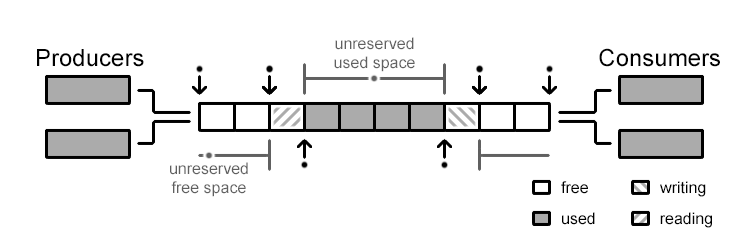
\includegraphics[width=0.80\textwidth]{images/ring.png}
    \caption{Struttura di un \textit{Ring Buffer}}
    \label{fig:ring_buffer}
\end{figure}

Le dimensioni dei ring buffer sono state calibrate sui worst case attesi:

\begin{itemize}
    \item \textbf{Board A, canale PC}: 8\,192 byte. Anche se l'immagine completa è di 36\,864 byte, l'applicazione consuma i byte in tempo reale via \texttt{read\_byte\_pc}, quindi il buffer accumula solo l'eventuale burst di byte arrivati tra una lettura e l'altra. 8~KB è un compromesso ampio.
    \item \textbf{Board A, canale b2b}: 256 byte. Sufficiente per le brevi risposte di tipo \texttt{TYPE\_TEXT} o \texttt{TYPE\_ACK} provenienti da Board B (poche decine di byte).
    \item \textbf{Board B, canale b2b}: 8\,199 byte. Pari a 8\,192 byte del crop più 7 byte di header del frame, in modo da poter assorbire un intero messaggio anche se l'applicazione fosse momentaneamente impegnata.
\end{itemize}

\section{Formato del frame}
\label{sec:frame-format}
Su un canale seriale orientato a flusso di byte, è necessario un protocollo di livello applicativo per delimitare i messaggi e identificarne il tipo. Il protocollo adottato in questo progetto utilizza un frame a lunghezza fissa di 7 byte di intestazione seguito da un payload di lunghezza variabile, come mostrato in Figura \ref{fig:protocollo}.

\begin{figure}[H]
    \centering
    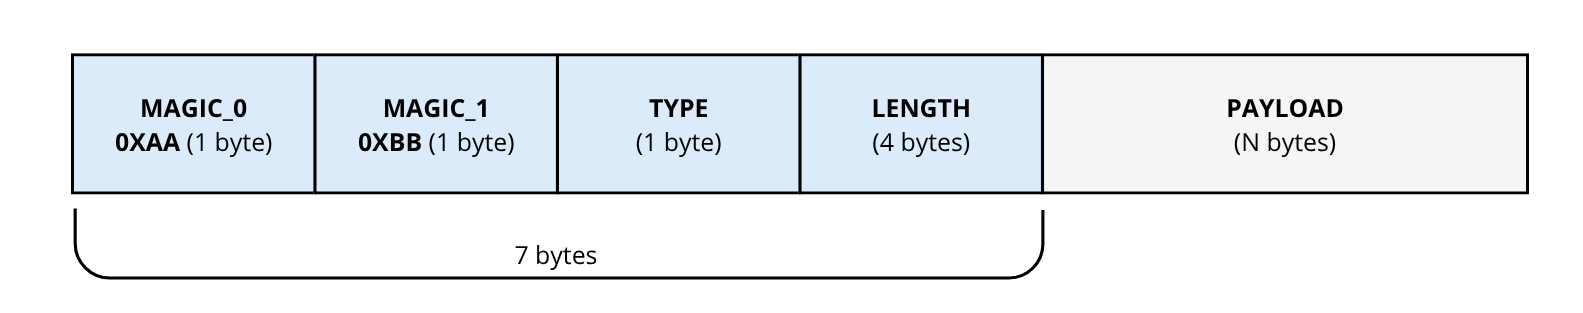
\includegraphics[width=0.95\textwidth]{images/protocollo_comunicazione.png}
    \caption{Struttura di un frame del protocollo applicativo}
    \label{fig:protocollo}
\end{figure}



I primi due byte (\textit{magic number}) costituiscono una sequenza di sincronizzazione: in ricezione, il parser scarta tutti i byte ricevuti finché non incontra la coppia $\mathtt{0xAA\,0xBB}$, dopodiché interpreta il byte successivo come tipo di messaggio. Il campo \texttt{TYPE}, di un singolo byte, identifica la natura del payload secondo la tabella dei tipi definiti per il protocollo (Tabella~\ref{tab:msg-types}). Il campo \texttt{LENGTH}, di 4 byte in \textit{big-endian}, indica la dimensione del payload che segue.

\begin{table}[H]
    \centering
    \caption{Tipi di messaggio definiti dal protocollo.}
    \label{tab:msg-types}
    \begin{tabular}{clll}
        \toprule
        \textbf{Codice} & \textbf{Nome} & \textbf{Direzione} & \textbf{Significato} \\
        \midrule
        $\mathtt{0x01}$ & \texttt{TYPE\_GRAY} & PC $\rightarrow$ A & Immagine grayscale da analizzare \\
        $\mathtt{0x02}$ & \texttt{TYPE\_BBOX} & A $\rightarrow$ PC & Bounding box (riservato, non usato) \\
        $\mathtt{0x03}$ & \texttt{TYPE\_ACK}  & A $\rightarrow$ PC, B $\rightarrow$ A & Sistema pronto \\
        $\mathtt{0x04}$ & \texttt{TYPE\_ERR}  & varie & Notifica di errore (codice in payload) \\
        $\mathtt{0x05}$ & \texttt{TYPE\_NONE} & A $\rightarrow$ PC & Nessuna targa rilevata \\
        $\mathtt{0x06}$ & \texttt{TYPE\_CROP} & A $\rightarrow$ B & Crop della targa per OCR \\
        $\mathtt{0x07}$ & \texttt{TYPE\_TEXT} & B $\rightarrow$ A $\rightarrow$ PC & Stringa di caratteri riconosciuta \\
        \bottomrule
    \end{tabular}
\end{table}

\section{Implementazione dei primitivi}
\label{sec:primitivi}

L'invio e la ricezione di un frame sono incapsulate in due primitive simmetriche, \texttt{send\_msg\_on} e \texttt{recv\_msg\_on}, parametrizzate dalle funzioni di lettura/scrittura del canale specifico (PC o b2b). In invio, la primitiva scrive in sequenza i due magic byte, il tipo, i quattro byte di lunghezza e infine il payload (Listato~\ref{lst:send}). In ricezione, la routine cerca prima la coppia di magic, legge il tipo e la lunghezza, e infine legge esattamente \texttt{size} byte di payload nel buffer fornito dal chiamante.

\begin{lstlisting}[style=stileC, caption={Primitiva generica per l'invio di un frame.}, label={lst:send}]
static void send_msg_on(void (*wb)(uint8_t),
                        void (*wbuf)(const uint8_t *, uint32_t),
                        uint8_t type, const uint8_t *payload, uint32_t len)
{
    wb(MAGIC_0); wb(MAGIC_1); wb(type);
    wb((len >> 24) & 0xFF);
    wb((len >> 16) & 0xFF);
    wb((len >>  8) & 0xFF);
    wb( len        & 0xFF);
    if (payload && len > 0) wbuf(payload, len);
}
\end{lstlisting}

L'uso di due puntatori a funzione consente al firmware di Board A di gestire i due canali (PC e Board B) con la stessa logica, differenziandoli solo per le primitive di byte. Sono definite due macro \texttt{send\_msg\_pc} e \texttt{send\_msg\_b2b} che istanziano la primitiva con le funzioni corrette per ciascun canale.

\section{Sincronizzazione di boot}
\label{sec:sync-boot}

All'accensione, le due schede non sono in uno stato consistente: la Board B impiega circa 500~ms a inizializzare la rete neurale, mentre Board A potrebbe terminare la propria inizializzazione prima che B sia pronta a ricevere. Se in questo intervallo il PC inviasse un'immagine, la Board A potrebbe accettarla, eseguire l'inferenza YOLO e tentare di inoltrare il crop a una Board B non ancora pronta, con il rischio di bloccare l'intero sistema.

Per evitare questa condizione di gara, è stato implementato un meccanismo di \textit{handshake} a due livelli:

\begin{enumerate}
    \item All'avvio, Board B termina l'inizializzazione della propria rete OCR e invia immediatamente un messaggio \texttt{TYPE\_ACK} sulla USART2 verso Board A.
    \item Board A, dopo aver inizializzato a sua volta la rete YOLO, si mette in attesa bloccante di un messaggio dalla USART2. Solo quando riceve l'ACK da B, la Board A invia il proprio \texttt{TYPE\_ACK} al PC sulla USART3.
    \item Lo script Python sul PC attende il primo messaggio dalla porta seriale e procede solo dopo aver ricevuto \texttt{TYPE\_ACK}. A questo punto inizia il ciclo di invio delle immagini.
\end{enumerate}

In questo modo la prima immagine viene inviata solo quando entrambi i microcontrollori hanno completato il proprio bring-up. Il meccanismo si comporta correttamente anche se le due schede vengono accese in ordine arbitrario, perché il timing assoluto non conta: ciò che conta è l'ordine causale degli ACK lungo la catena B~$\rightarrow$~A~$\rightarrow$~PC.
